\section{Superposition as a Cause of Hallucinations}
\label{sec:superposition_as_a_cause_of_hallucinations}

A key question from the paper was whether interference from superposition causes hallucinations in large language models.
To test this, we trained a classifier on high-sparsity data, inducing superposition, and evaluated it on low-sparsity data.

\subsection{Dataset}
We used a dataset with five features, represented by English affixes: \textit{un-}, \textit{re-}, \textit{-able}, \textit{-ful}, \textit{-ness}, although any set of affixes could work.
Two datasets were generated: one with words containing a single affix (pure words) and another with words containing multiple affixes (dual words, e.g., \textit{unreliable}).
The pure dataset was split into training and test sets, while the dual dataset was reserved for evaluation.

\subsection{Model}
We trained a model with an embedding layer, a convolutional layer, a hidden layer, and ReLU activation.
The hidden layer had only two neurons, forcing it to use superposition to encode all five features.

\subsection{Results}
Using the \href{https://colab.research.google.com/github/anthropics/toy-models-of-superposition/blob/main/toy_models.ipynb}{toy model framework}, we visualized the five features in the hidden layer.
\begin{figure}[h]
	\centering
	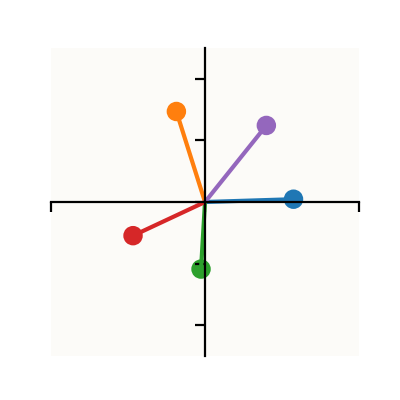
\includegraphics[width=0.3\linewidth]{figures/hallucinations_hidden_layer.png}
	\caption{Representation of the five features in the hidden layer.}
	\label{fig:hidden_layer_representation}
\end{figure}
Figure \ref{fig:hidden_layer_representation} shows the model all features, though it didn't form the pentagon-like structure noted in the paper.
Table \ref{tab:hallucinations_results} shows the results for the test set and the dual dataset.
\begin{table}[h]
	\centering
	\begin{tabular}{lc}
		\toprule
		\textbf{Dataset} & \textbf{Accuracy} \\
		\midrule
		Test set         & 0.9772            \\
		Dual dataset     & 0.9581            \\
		\bottomrule
	\end{tabular}
	\caption{Model evaluation on the test set and the dual dataset.}
	\label{tab:hallucinations_results}
\end{table}
The model performed well on the test set, but accuracy dropped on the dual dataset, even though each dual word had twice the correct labels.
This suggests that when features are less sparse than in training, the additive interference from superposition may cause misinterpretations, contributing to hallucinations in large language models.
